\begin{figure*}[tp] 
\vspace{-0. in}
\centering
\centerline{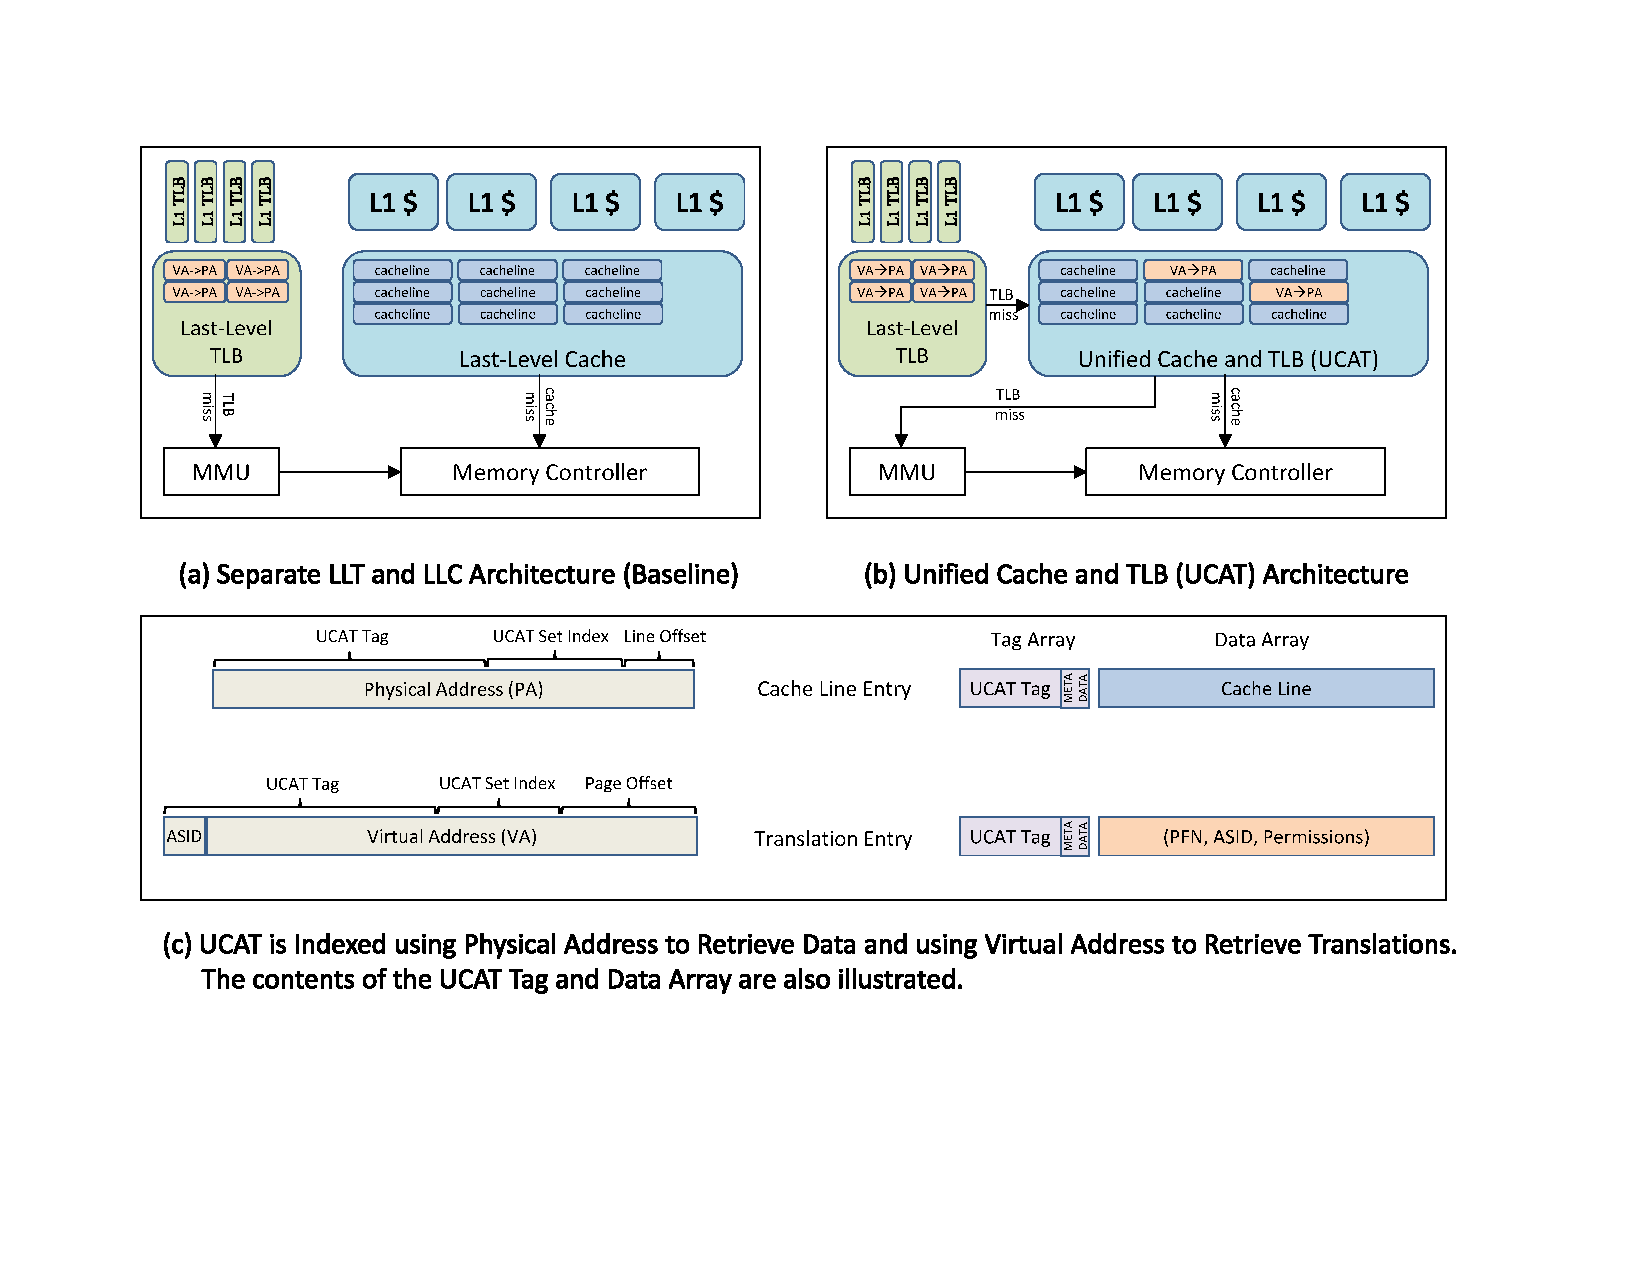
\psfig{file=FIGURES/UCAT,scale=0.80,width=\textwidth}}
\caption{\small UCAT Architecture. \normalsize}
\label{fig:pagetable_placement} 
\vspace{-0.0in}
\end{figure*}

\section{Unifying Caches and TLBs}
\label{sec:UCAT}

\noindent Modern chip multiprocessors use a multi-level TLB and cache
hierarchy to ensure high performance. The last-level in each hierarchy
is architected as a single large unified structure (holding both
instruction and data entries) that is shared across all cores. For
example, the unified last-level cache (LLC) contains several hundred
thousand cache lines\footnote{An 8MB cache with 32B lines contains
256K cache lines.}) that store data for recent memory references.
Similarly, the unified last-level TLB (LLT) contains 512-1024 TLB
entries~\cite{} that store address translations for recent memory
references.

The LLT and LLC are architected using a tag array and a data array.
The LLT tag array stores a virtual address while the LLC tag array
stores a physical memory address.\footnote{Additional meta data (e.g.
coherence state, replacement state, etc) is also stored in the tag
array.}. On the other hand, the LLT data array stores the physical
address corresponding to the virtual address translation (roughly 8
bytes) while the LLC data array stores a copy of the data from memory
at a cache line granularity (e.g. 32-64 bytes).

The LLT and LLC are cache structures with similar sized tag arrays.
Since they provide different types of data, there is a 4x-8x
difference in the data array size. We observe that, since the LLC data
array is greater than the LLT data array, the LLC can also serve as
gigantic TLB with as many entries as there are LLC lines. As such, the
conventional LLC can potentially be used to store virtual to physical
translations just like a TLB (in addition to caching data from
memory). Based on this insight, we propose to re-architect the
conventional LLC as a {\em Unified Cache and TLB (UCAT)}.

\subsection{UCAT Architecture}

\noindent A Unified Cache and TLB (UCAT) holds both cache lines and
TLB entries in a single hardware structure. Thus, a UCAT-entry is
either a cacheline or a TLB-entry. A single-bit per UCAT-entry can be
used to distinguish between the two.

In the baseline system where a UCAT-entry only stores a cache line,
the tag-array stores the physical address while the data array stores
the cache line (e.g. 32-bytes). However, when the UCAT-entry serves as
a TLB-entry, the UCAT tag-array stores the virtual address while the
data-array stores the virtual to physical address translation (roughly
8 bytes). At first, it may appear as though a large fraction of the
UCAT-entry is being wasted (e.g. 24-bytes out of a 32-byte line in our
baseline). However, recent studies have shown (and independently
verified in this study) that the majority of LLC entries are unused
after cache insertion~\cite{}. In other words, the existing LLC
entries are already inefficiently utilized. UCAT efficiently utilizes
the conventional LLC space by storing TLB entries in addition to cache
lines.

Figure X illustrates how a physical address maps to a UCAT set to
store/retrieve a cache line (baseline). Similarly we illustrate how a
virtual address maps to a UCAT set to store/retrieve a TLB entry.

% \subsection{Static UCAT Partitioning}
% 
% \noindent UCAT entries must be distributed between TLB-entries and
% cachelines. One way of accomplishing this is by statically employing
% {\em way partitioning}~\cite{}. With {\em N} ways in a UCAT set, {\em
% m} ways are statically devoted to cachelines while the remaining {\em
% N-m} ways are statically devoted to TLB entries. Cachelines are only
% inserted in the ways to devoted to them while TLB entries are inserted
% in the ways devoted to them. When evicting UCAT entries, a replacement
% policy is used (e.g. LRU, RRIP) to select between candidates within
% the same UCAT partition. We refer to this design as {\em Static UCAT
% Partitioning (UCAT-S)}.
% 
% Profiling across various workloads for different values of {\em m} can
% help arrive at the best UCAT partition for cachelines and TLB entries.
% Figure X illustrates the behavior for different {\em m}.

\begin{figure}[tp] 
  \vspace{-0.in} \centering
  \centerline{\psfig{file=GRAPHS/UCAT_perf,angle=-90,width=\columnwidth}}

  \caption{\small Performance of DRAM-TLBs. \normalsize}
  \label{fig:perf_UCAT} 
  \vspace{0.2 in}
\end{figure}

\begin{figure}[tp] 
  \vspace{0.in} \centering
  \centerline{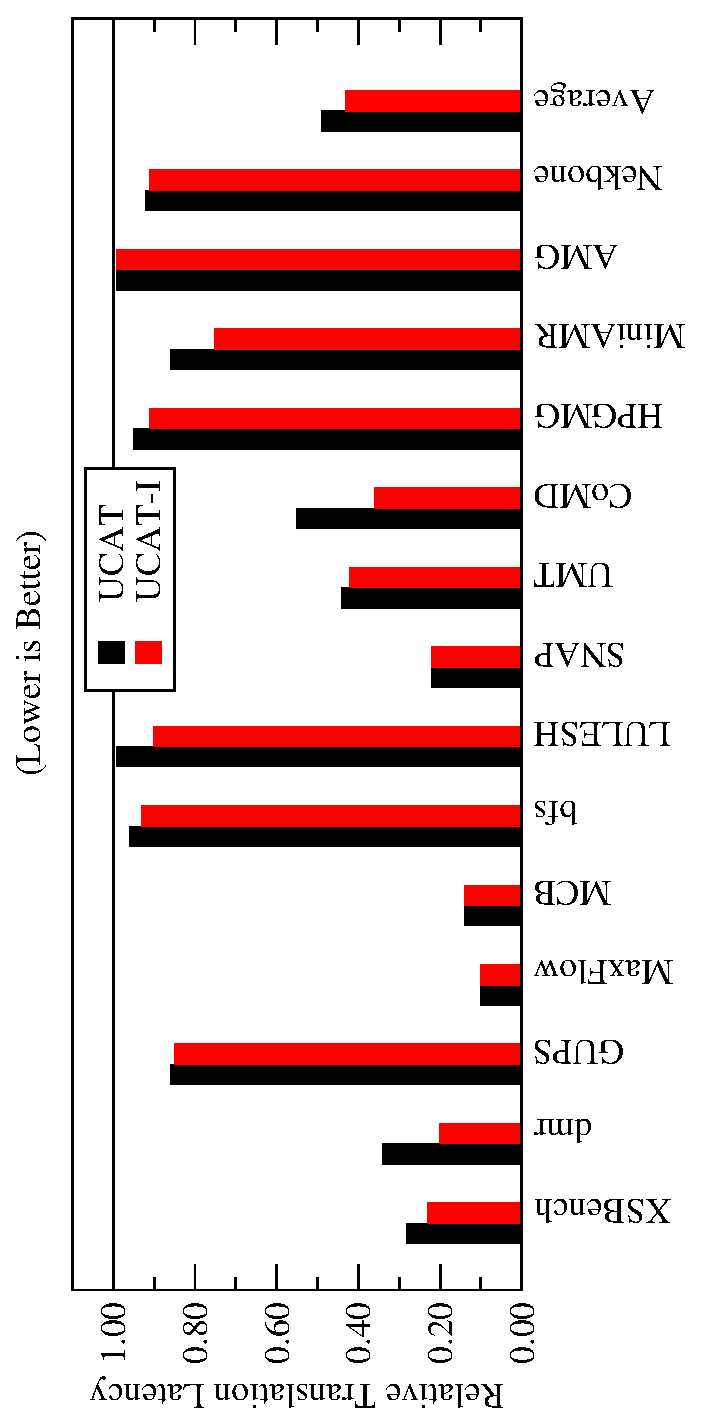
\psfig{file=GRAPHS/UCAT_tlblat,angle=-90,width=\columnwidth}}

  \caption{\small TLB miss penalty relative to baseline system.\normalsize}
  \label{fig:tlblat_UCAT} 
  \vspace{-0.1 in}
\end{figure}

\begin{figure}[tp] 
  \vspace{0.in} \centering
  \centerline{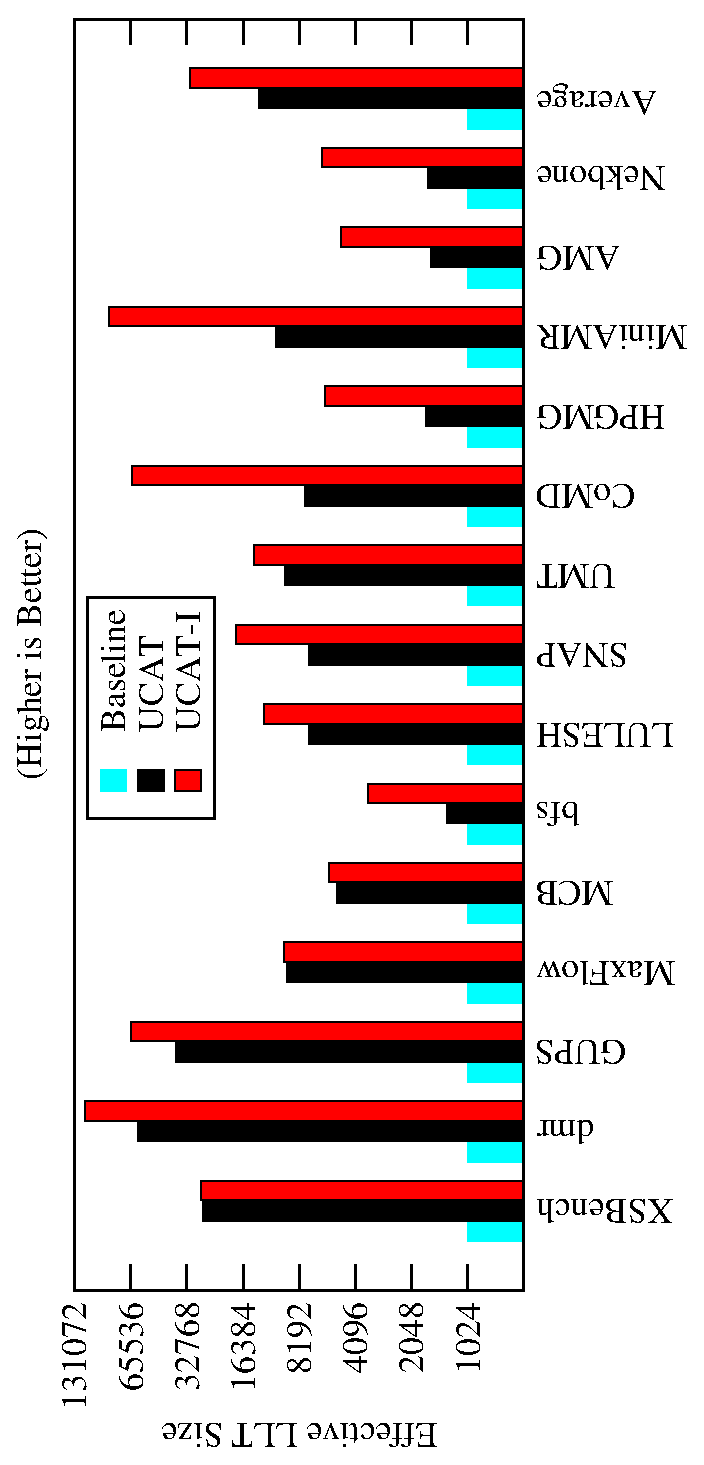
\psfig{file=GRAPHS/UCAT_tlbsize,angle=-90,width=\columnwidth}}

  \caption{\small Effective TLB Size.\normalsize}
  \label{fig:tlblat_UCAT} 
  \vspace{-0.1 in}
\end{figure}

\subsection{UCAT Allocation and Management}

% PUCAT is inefficient when the TLB-entries and cachelines have
% different capacity requirements at run time. To address this problen,
TLB-entries and cachelines dynamically share the entries in a UCAT
set. With this approach, TLB-entries and cachelines contend with one
another to occupy UCAT space. As in the baseline LLC, a single
replacement policy is used to manage UCAT entries in a set. UCAT hits
update the replacement state appropriately while UCAT misses utilize
the conventional replacement policy to select the victim candidate
within the set.

Figure Y shows UCAT performance.

The baseline polic UCAT allocates entries based on demand, rather than
utility. As such, workloads that requently stream through a large
number of cache lines can constantly discard UCAT TLB entries. Thus,
we propose to enhance DUCAT by improving the underlying replacement
policy. Our baseline system uses the Dynamic Re-Reference Interval
Prediction (DRRIP) replacement policy~\cite{}. In this baseline
policy, all UCAT insertions follow the same re-reference prediction
(i.e. insertion policy). We propose to enhance the insertion policy
for TLB entries by inserting them with a {\em near-immediate
prediction} rather than the baseline {\em far prediction}. In doing
so, TLB entries are allowed to reside in the UCAT for a longer
duration. We refer to this enhancement as {\em UCAT with Insertion
(UCAT-I)}.

Figure Y also shows performance of UCAT-I.

\begin{figure*}[t] 
  \vspace{-0. in} \centering
%  \centerline{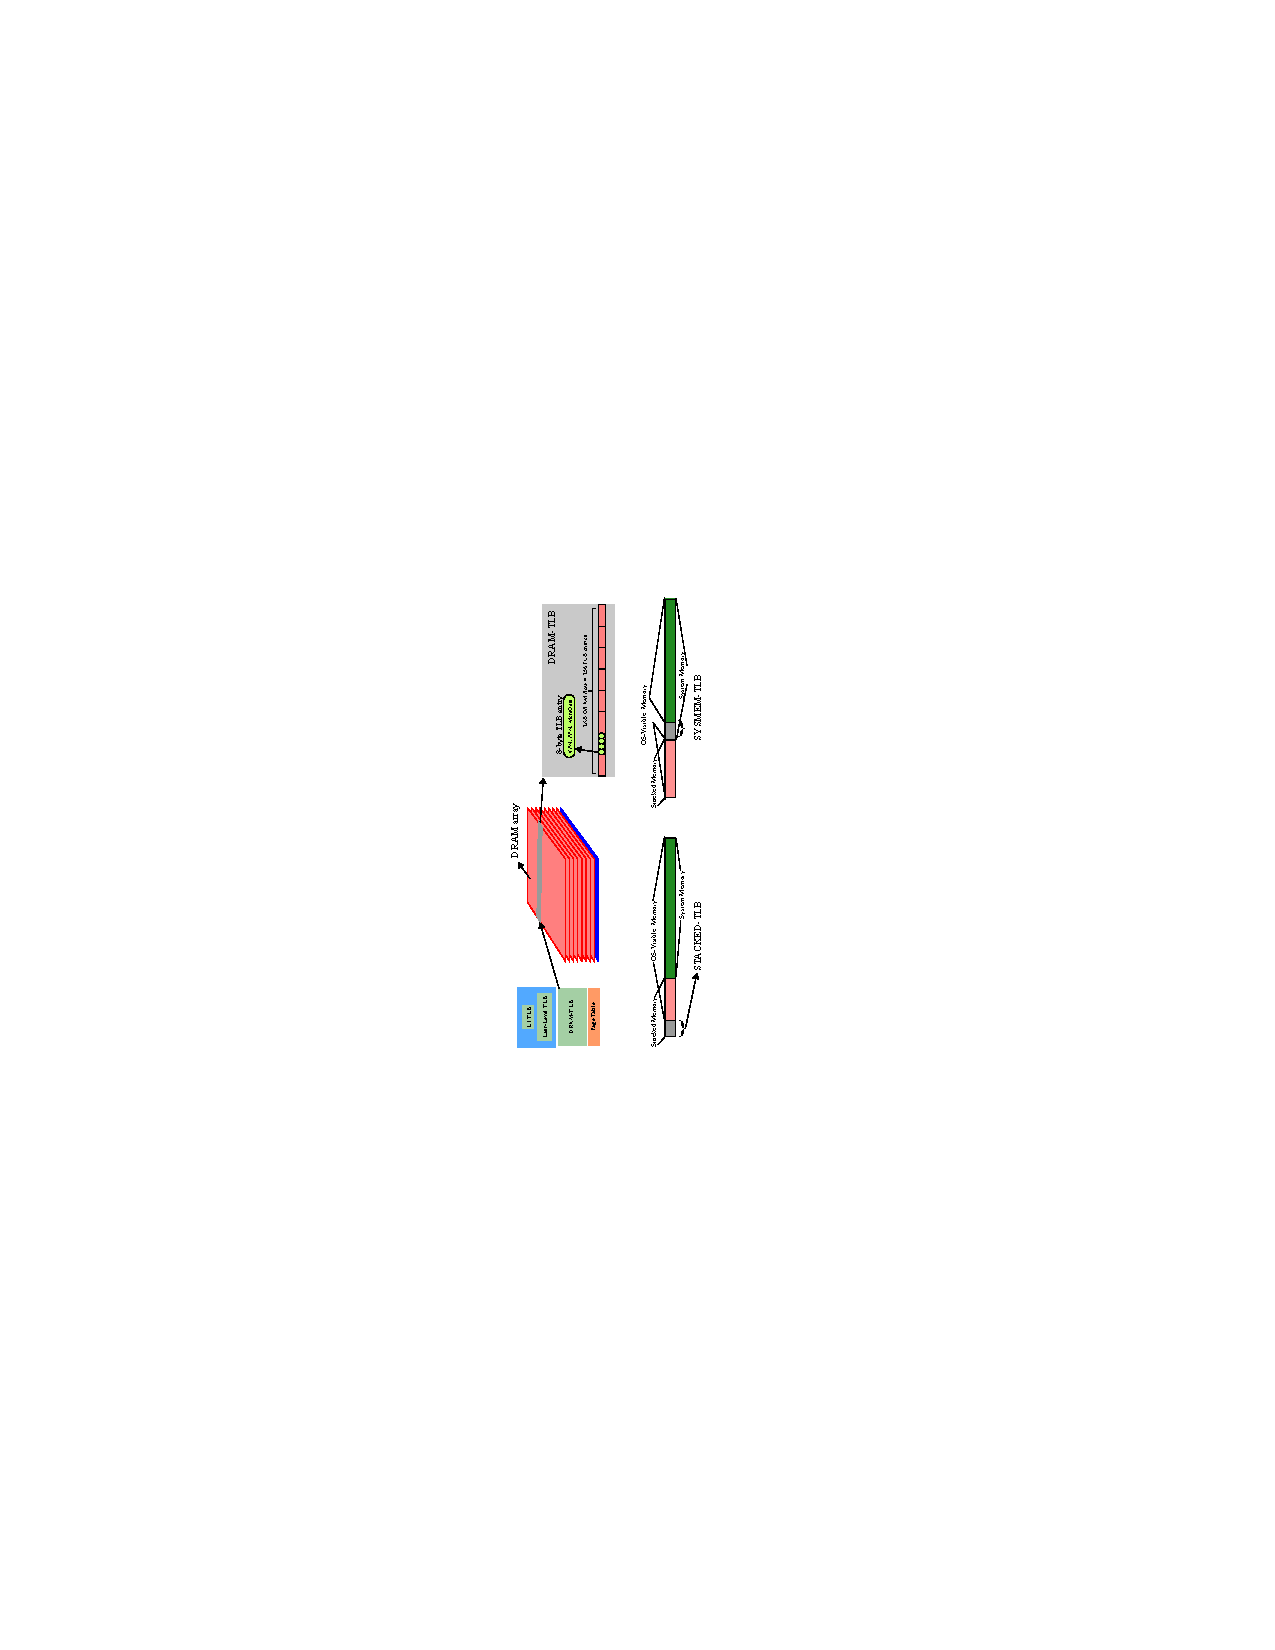
\psfig{file=FIGURES/stacked_tlb,angle=-90,width=\columnwidth}}
   \centerline{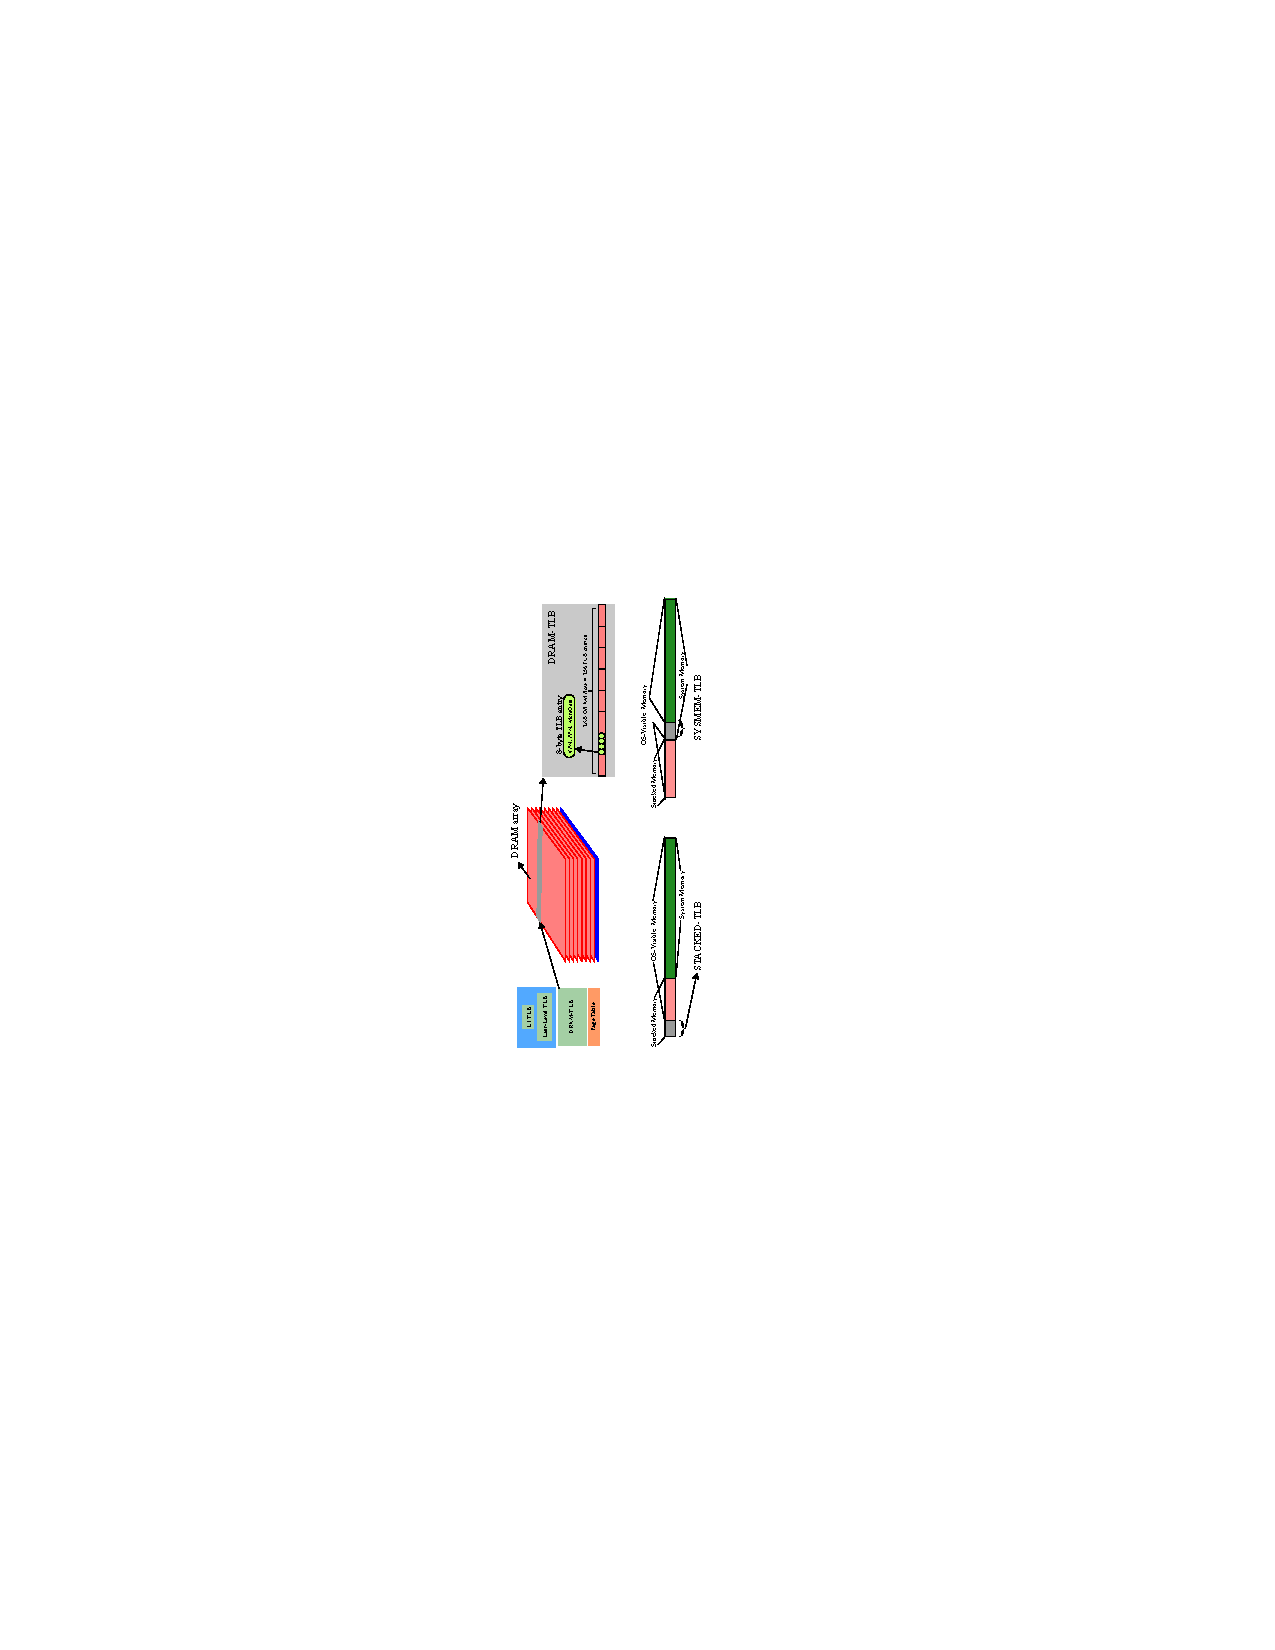
\psfig{file=FIGURES/stacked_tlb,width=\textwidth}}

  \caption{\small Improving TLB coverage by embedding TLBs in DRAM
    (DRAM-TLB). A DRAM-TLB architected using commodity DRAM is called
    SYSMEM-TLB and a DRAM-TLB architected with stacked DRAM is called
    Stacked-TLB. \normalsize}
  \label{fig:stacked_tlb} 
  \vspace{-0. in}
\end{figure*}

\subsection{UCAT Optimizations}

To avoid this additional storage overhead, we propose using the
UCAT-entry status bits (i.e. MESI bits) to make the distinction.
Specifically, we insert TLB-entries into UCAT with the {\em exclusive}
and {\em shared} status bits to be valid. Note that cachelines can
either be in exclusive state or shared state, but not both.

